\section{Evaluation}
\subsection{End-to-End Performance}
% In this section, we mainly compare the wall-clock on-device training time and the test accuracy of \sys to baselines under various models, datasets and devices.

% \noindent \textbf{\sys reduces on-device training time significantly without compromising the test accuracy.}
\noindent \textbf{Overall performance.}
We begin with comparing the overall performace of \sys to its baselines.
We conduct the experiments on 3 various NN architectures and 4 various downstream datasets. 
The details are mentioned in $\S$\ref{sec:impl}.
We record the test accuracy every epoch and report the best test accuracy and corresponding wall-clock training time.
The computing cost on testing is excluded.
Table ~\ref{table-e2e accuracy} shows the best test accuracy.
\sys does not compromise test accuracy compared to its baselines.
As is shown in Figure ~\ref{fig:e2etime}, by dynamically routing training data to lightweight subnets, \sys achieves up to 6.60$\times$ speedup over all baselines, and 1.47$\times$--2.52$\times$ speedup compared to \texttt{PET}. 
% Specifically, \sys achieves 
Here we perform a detailed analysis:
\begin{itemize}[leftmargin=10pt,topsep=0pt]
\item \textit{Compared to \texttt{FT-All}.}
\sys significantly outperforms \texttt{FT-All} by up to 6$\times$.
This comes from both the parameter efficiency and our key designs.
\item \textit{Compared to \texttt{PET}.}
\sys consistently outperforms \texttt{PET} by up to 2.5$\times$.
This is attributed to the full utilization of data diversity.
\item \textit{Compared to other strong baselines (\texttt{PT}/\texttt{ET}).}
\sys also outperforms these strong baselines.
\texttt{PT}'s NN approximation only reduces training FLOPs, which does not translate to wall-clock time reduction on general-purpose processors.
\texttt{ET} only performs tensor-level non-deterministic training with evaluated importance. It cannot fully utilize the potential of NN approximation and data diversity.
Another significant drawback is that they compromise parameter efficiency, preventing them from enjoying various benefits of PET in terms of both training and deployment mentioned in $\S$\ref{subsec:PET}.
\end{itemize}

% \noindent $\bullet$ \textit{\sys v.s. FT-All/PT/ET.}
% FT-All is time-consuming without parameter-efficiency and NN approximation.
% PT online approximates the network during on-device training but with extra pruning overhead.
% % It achieves similar performance to FT-All.
% ET only partially benefits from parameter-efficiency.
% Therefore, \sys can achieve significant improvements (up to 6.1$\times$/6.6$\times$/3.9$\times$ on 3 networks with various PET methods) compared to these baselines.

% \noindent $\bullet$ \textit{\sys v.s. PET.}
% \sys outperforms PET by 1.47$\times$--2.52$\times$.
% These numbers come from NN approximation of \sys, and are influenced by PET settings.


\noindent \textbf{Performance under various accuracy budgets. }
In practice, on-device training tasks often do not choose to reach the highest test accuracy because of the marginal effect.
Thus, we also explore the wall-clock training time for different accuracy targets.
Figure ~\ref{fig:time2acc} shows the time-to-accuracy curve of \sys and its baselines.
We observe that, thanks to our dynamic routing design, \sys achieves shorter per-epoch computation time and faster end-to-end convergence speed.
Further, we report the speedup achieved by \sys when reaching 85\%/90\%/95\%/99\% of the baseline's best accuracy.
As is shown in Figure ~\ref{fig:speedup2acc}, \sys always achieves significant speedup (1.86$\times$/1.89$\times$/1.54$\times$/1.80$\times$ to \texttt{PET}, and 4.17$\times$/4.20$\times$/5.43$\times$/5.82$\times$ to \texttt{FT-All}) under different accuracy budges.
Specifically, there is a trend that the higher the target accuracy, the greater the speedup achieved by \sys.
This is because, as training progresses, more and more data require fewer computational resources, allowing \sys to effectively mitigate the marginal effect of training.

\noindent \textbf{Performance on various devices.}
We further explore the performance of \sys on 3 devices: Jetson TX2, Raspberry Pi 4B and MI 10 smartphone in Figure ~\ref{fig:crossdevice}.
\sys outperforms its baselines on all these devices by a minimum factor of 1.61$\times$/1.63$\times$/1.72$\times$, and the improvements are particularly notable on both GPU-empowered devices (e.g., Jetson TX2) and resource-constrained devices (e.g., Raspberry Pi 4B and MI 10 smartphone).

\noindent \textbf{Performance in extremely few-shot scenarios.}
We also explore the performance of \sys with extremely few human-labeled training data in Table \ref{table-fewshot}. 
Our system consistently outperforms the baseline method under 5-shot/10-shot settings.
We further apply a commonly used few-shot learning approach: pseudo-labeling~\cite{lee2013pseudo}. 
We provide 100 pseudo-labeled data for each category. 
\sys significantly outperforms the baseline and achieves accuracy close to training with adequate human-labeled data.

% Specifically, \sys is friendly to AI accelerators (NPUs) designed for NN inference, making on-device fine-tuning practical and even efficient.
\begin{table}[!t]
\caption{Performance in extremely few-shot scenarios. PL: Pseudo Labeling; Model: ResNet50; Dataset: DTD Device: Jetson TX2.}
\label{table-fewshot}
\centering
\footnotesize
\begin{tabular}{@{}ccccccc@{}}
\toprule
                     & \multicolumn{3}{c}{\textbf{FT-All}} & \multicolumn{3}{c}{\textbf{\sys}} \\ \cmidrule(l){2-7} 
                     & 5-shot      & 10-shot     & PL      & 5-shot     & 10-shot     & PL     \\ \midrule
\textbf{Time (min.)} & 7.92          & 16.38          & 138.21     & 3.60         & 5.97          & 35.53    \\
\textbf{Accu. (\%)}   & 12.92          & 27.28          & 55.32      & 18.13         & 32.71          & 60.15     \\ \bottomrule
\end{tabular}
    
    
    
\end{table}

\begin{figure}[!t]
    \centering
    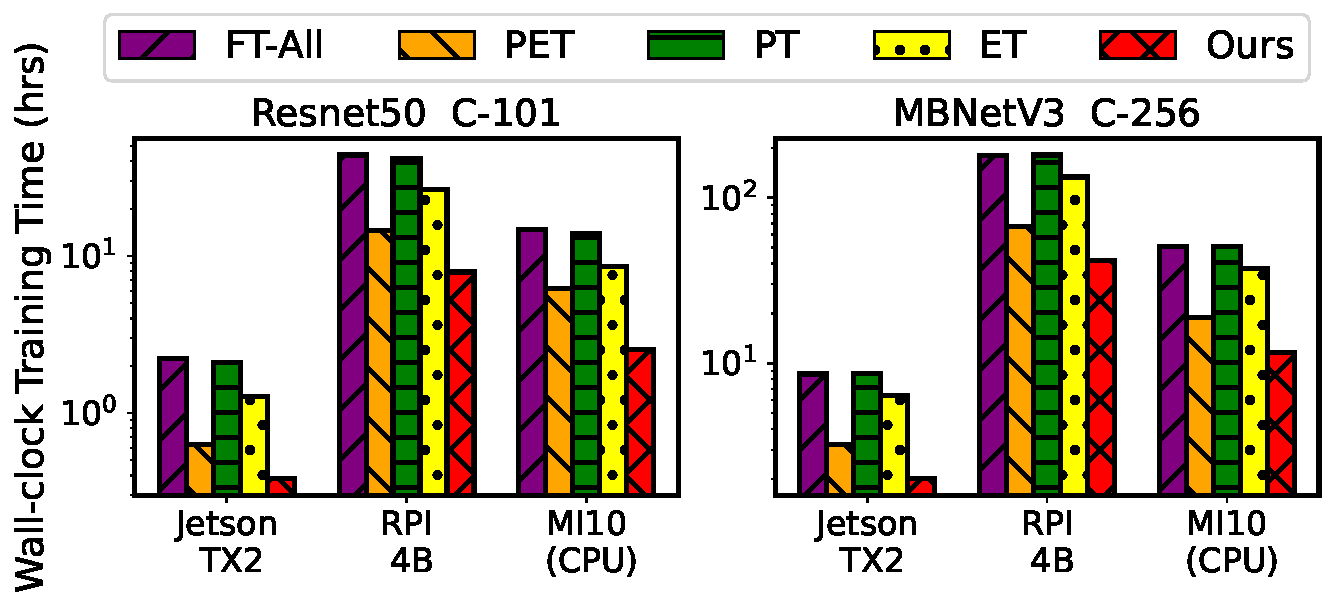
\includegraphics[width=0.96\linewidth]{figs/cross_devices.pdf}
    
    \caption{Performance on various devices.}
    
    \label{fig:crossdevice}
\end{figure}


\begin{figure}[!t]
    \centering
    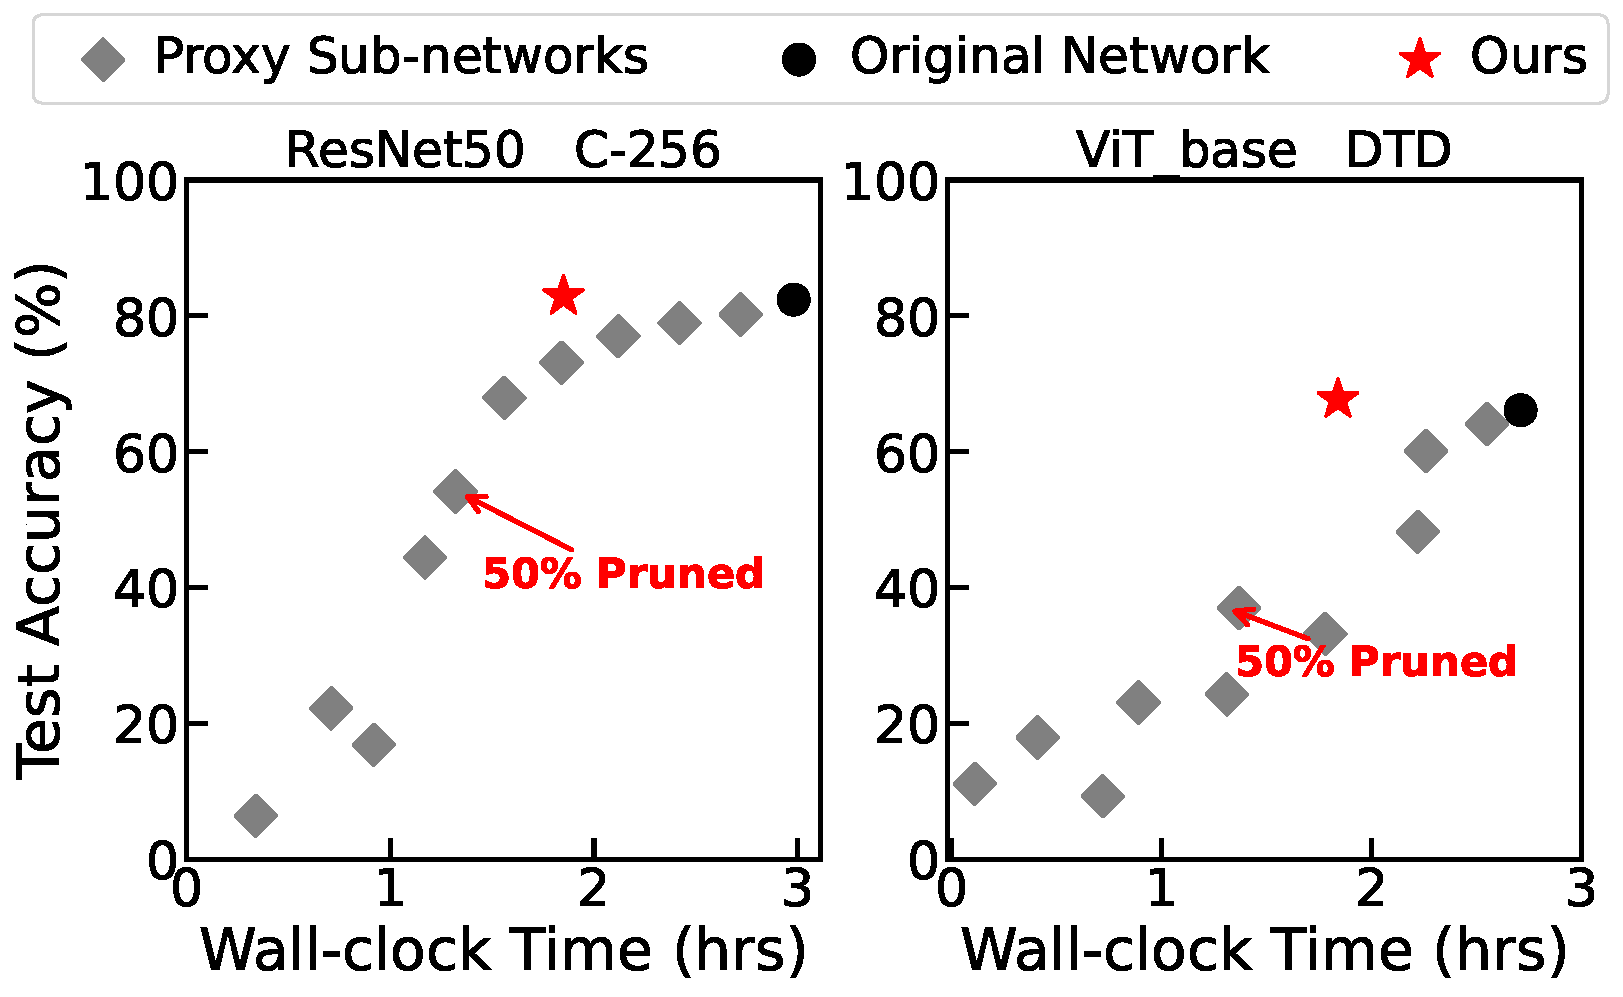
\includegraphics[width=0.76\linewidth]{figs/static.pdf}
    
    \caption{Compared to static alternative proxy sub-networks. Our data-aware subnet routing is a pareto-improved solution.}
    
    \label{fig:static}
\end{figure}



% \label{subsec:ablation}

\subsection{Design Effectiveness and Sensitivity Analysis}
\label{subsec: sensitivity}
In this section, our primary focus is on analyzing the effectiveness and sensitivity of \sys design.

\noindent \textbf{Compared to static alternative proxy sub-networks.}
We compare our data-aware subnet routing strategy ($\S$\ref{subsec:data-aware training}) to statically routing all training samples to the same proxy sub-network.
Figure ~\ref{fig:static} shows the best test accuracy and wall-clock training time of the original network ($\bullet$), the proxy sub-networks (\textcolor{gray}{\scriptsize $\blacklozenge$}) and our data-aware subnet routing (\textcolor{red}{$\star$}).
We have the following observations:

(1) \textit{A simple, static replacement strategy could result in nontrivial degradation of convergence accuracy.}
% As proxy sub-networks become lighter, their test accuracy rapidly decreases.
After pruning the original network by 50\%, ResNet50 experiences a 28.24\% decrease in test accuracy on the Caltech-256 dataset, and ViT\_base suffers a 29.11\% decrease in test accuracy on the DTD dataset.
There are two reasons behind this. 
One is that there is an error between the original network and the approximated subnet. 
The other is that, without a resource-intensive search, the pruned network structure may not be optimal.

\begin{figure}[!t]
    \centering
    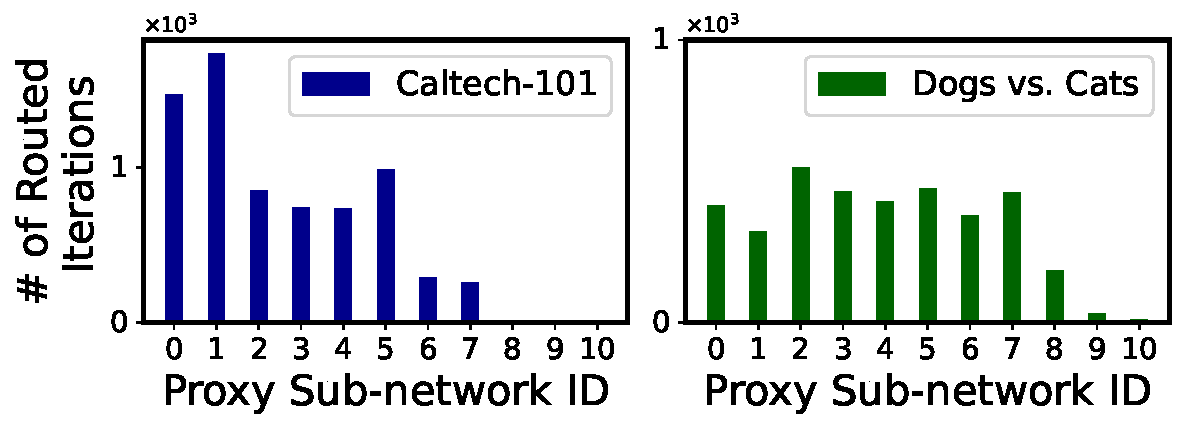
\includegraphics[width=0.82\linewidth]{figs/behavior.pdf}
    
    \caption{Behavior on datasets of different complexity.}
    
    \label{fig:behavior}
\end{figure}


(2) \textit{Our data-aware subnet routing is a pareto-improved solution.}
Compared to other static solutions, our approach not only reduces training time but also does not exhibit a noticeable decrease in accuracy.

\noindent \textbf{Behavior on datasets of different complexity.}
As is shown in Figure ~\ref{fig:behavior}, compared to the more complex dataset Caltech-101, \sys effectively routes more training samples to lighter subnets on Dogs vs. Cats dataset.

\noindent \textbf{Number of proxy sub-networks.}
Recall that we globally choose a proxy number $N$ = 10 (the pruning step size $d$ is about $1/N$).
Here we analysis the rationale and influence of choosing this factor.
As shown in Figure~\ref{fig:sensitivity}(a), a larger N provides more fine-grained approximation tradeoffs, but its benefit diminishes when large enough (e.g., >=10). 
Determining it properly isn't a challenge: \sys can provide heuristic suggestions to a typical range (e.g., 10--15); or the cloud can automatically obtain it through profiling on public dataset.

From our observation, the number of subnets does not apparently influence wall-clock training time (Figure~\ref{fig:sensitivity}(b), ResNet50+Caltech-256+TX2).
This is mainly because the size of the subnets already covers the entire trade-off space, regardless of the number $N$.

\noindent \textbf{Policy model training data.}
% \mwx{Add more explanations. In general, (1) data diversity is common characteristics that is more transferable. (2) large scale pretraining is the best way to capture this characteristic. (3) a severe OOD issue can be addressed by crowd-sourcing a portion of trainable data, federated learning the policy model or directly on-device continual training the policy model.}
\yws{
Recall that we train our policy model $\Omega$ on large scale public dataset, i.e. ImageNet.
Through the aforementioned end-to-end experiments, its effectiveness has been verified.
Here we discuss \sys's sensitivity to the data for capturing data difficulty.
We report fine-tuning ResNet50 on Caltech-101 dataset.
The data difficulty learned from the large-scale general dataset ImageNet exhibits a strong \textit{transferability}.
Figure~\ref{fig:sensitivity}(c) shows that training on ImageNet achieves comparable accuracy compared to directly training on Caltech-101.
When training policy model with 5\% data (simulating crowd-sourcing user-permitted training data), the policy model still can work well.
Only when the cloud training data completely mismatches with device data (e.g., using cifar-10 for training in Figure~\ref{fig:sensitivity}(c)), the policy model behaves biased.
}

\begin{table}[!t]
\caption{\yws{Significance of key designs.}}
\label{table:ablation}
\centering
\footnotesize
\setlength{\tabcolsep}{3pt}
\begin{tabular}{@{}L{0.42\linewidth}C{0.25\linewidth}C{0.25\linewidth}@{}}
\toprule
\textbf{Design} & \textbf{Training Time (h)} & \textbf{Test Acc. (\%)} \\
\midrule
\sys & 1.85 & 82.89 \\
W/O IDC pruning & N/A (shape mismatch) & N/A (shape mismatch) \\
W/O latent space alignment & 2.06 & 64.24 \\
W/O policy model based routing & 26.2 & 82.62 \\
\bottomrule
\end{tabular}
\end{table}

\noindent \textbf{Significance of key designs.}
% \mwx{IDC pruning, latent space alignment. has been discussed before. but make a summarization here.}
\yws{
In Table~\ref{table:ablation}, we show the significance of \sys's key designs.
We report fine-tuning ResNet50 on Caltech-256, Jetson TX2.
The results show that without IDC pruning, the proxy subnets cannot replace the original network because of shape mismatch.
Without latent space alignment, the pruned subnets conflict with each other, leading to a significantly dropped convergence accuracy.
Without the lightweight policy model for perceiving the data difficulty, the training is slowed down by over 13$\times$, because that \sys has to run each subnet to get and compare the extracted feature in each iteration.
}
\begin{figure}[!t]
    \centering
    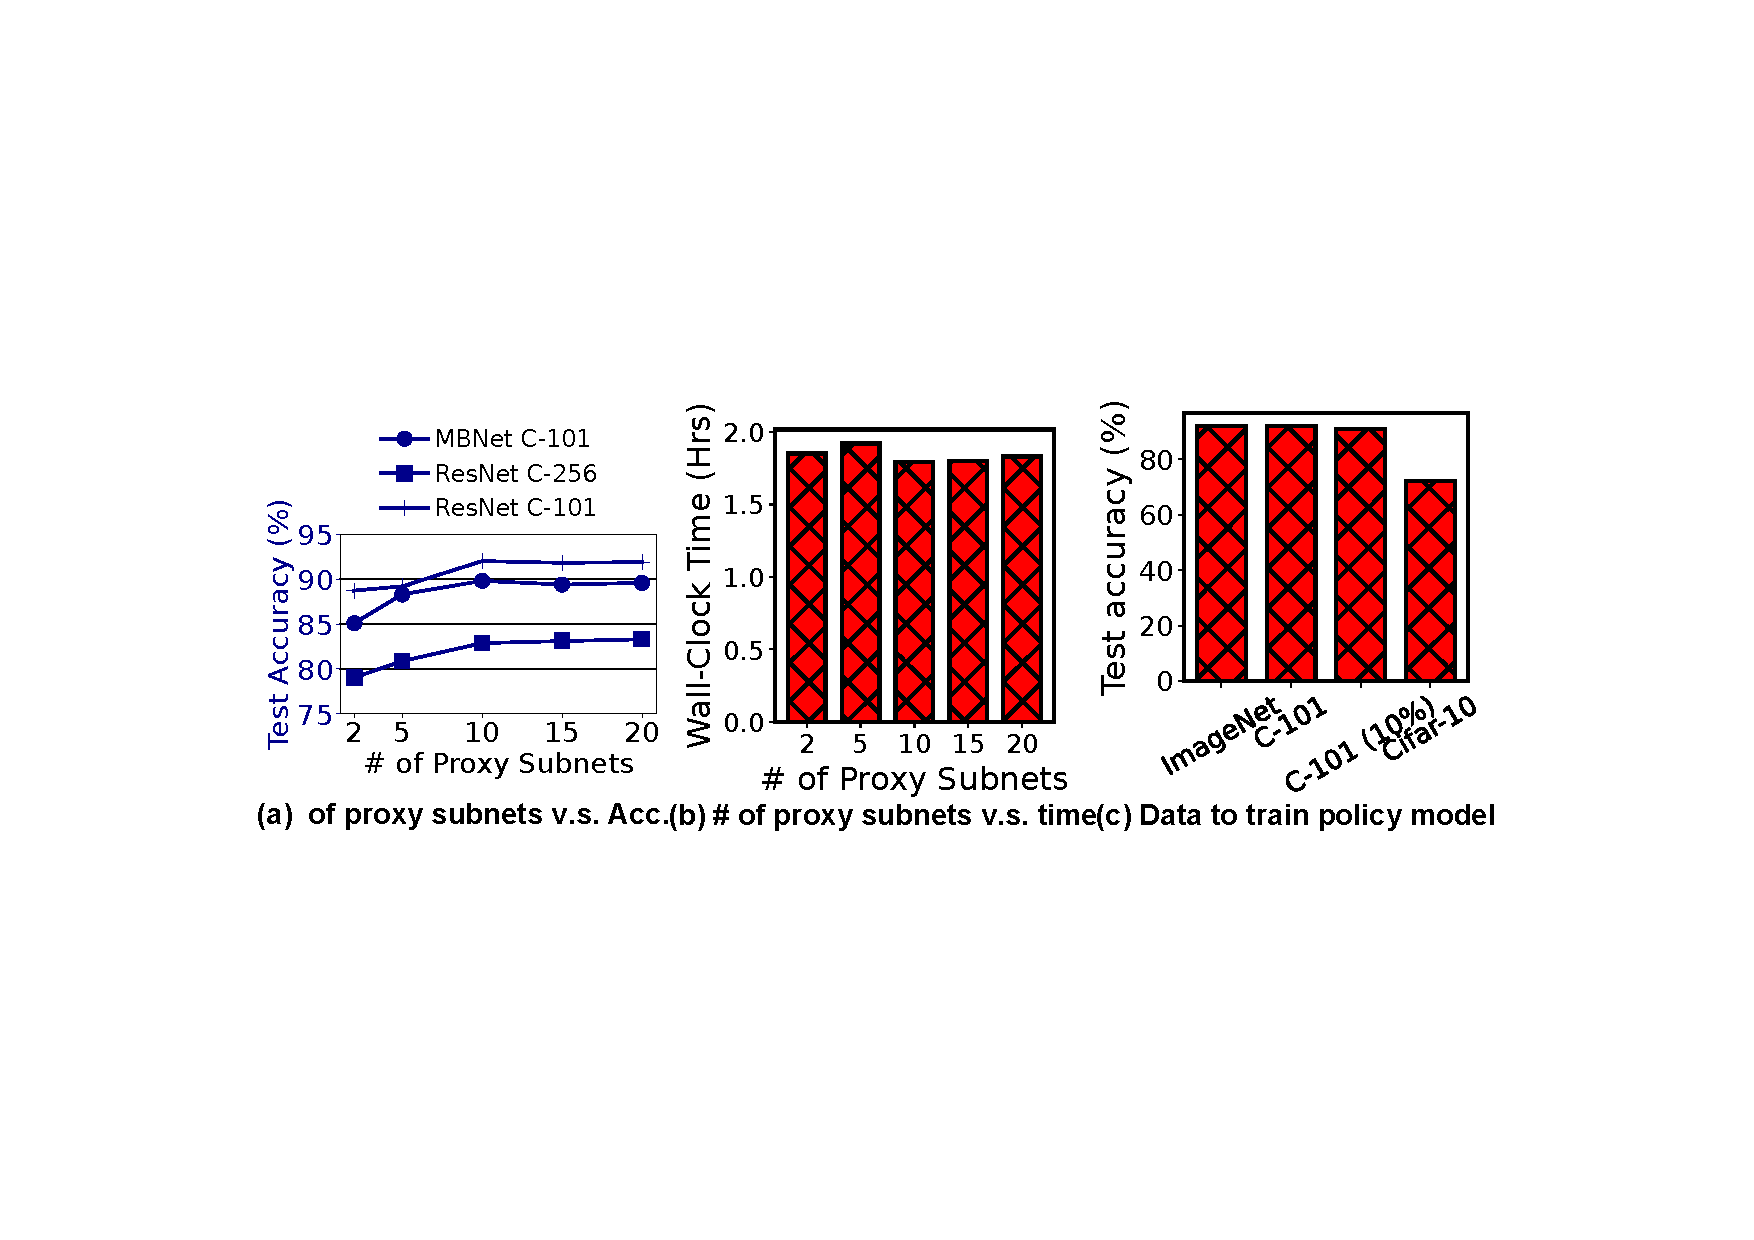
\includegraphics[width=0.98\linewidth]{figs/sensitivity.pdf}
    
    \caption{Sensitivity analysis.}
    
    \label{fig:sensitivity}
\end{figure}


\begin{figure}[!t]
    \centering
    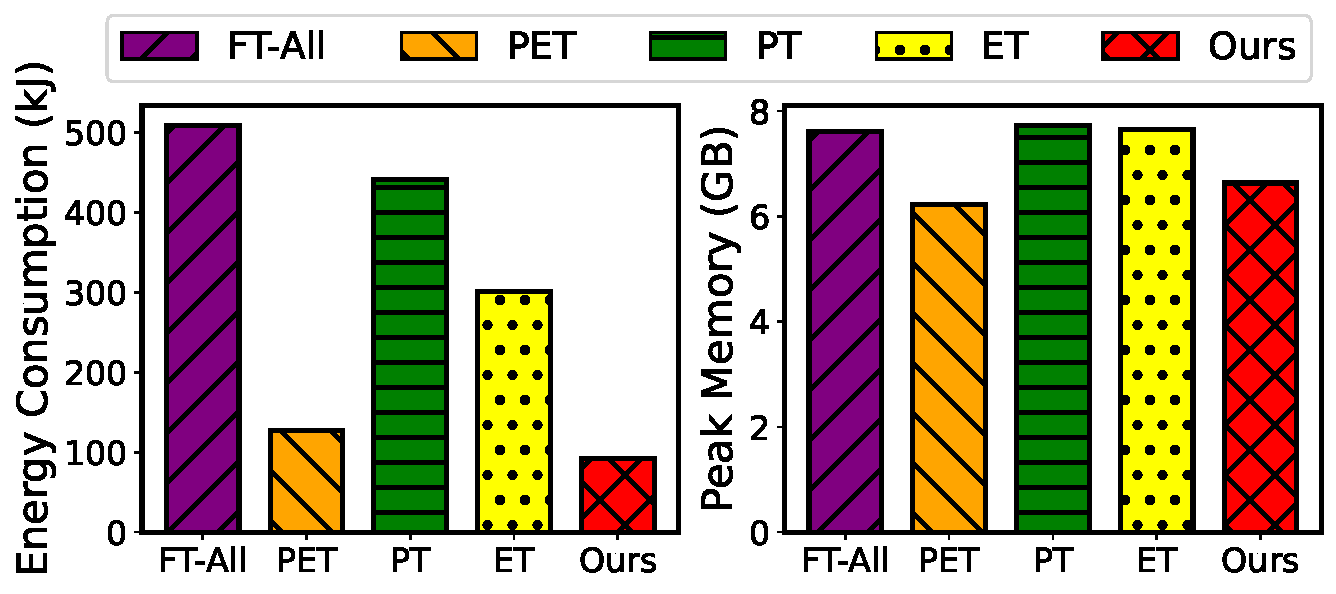
\includegraphics[width=0.82\linewidth]{figs/energyandmemory.pdf}
    
    \caption{Energy and memory consumption. }
    
    \label{fig:energy}
    \label{fig:memory and energy}
\end{figure}

\subsection{Energy and Memory Consumption}
\label{subsec: energy}
In this section, we report the energy and memory consumption of \sys against its baselines.
We train ResNet50 on Caltech-101 dataset with Jetson TX2.
We obtain energy/memory consumption by jtop~\cite{jtop}.
The results are shown in Figure~\ref{fig:energy}.

\noindent \textbf{Energy consumption.} 
\sys reduces energy consumption by 5.53$\times$/1.28$\times$ compared to \texttt{FT-All} and \texttt{PET}.
This is attributed to \sys's time efficiency, since \sys achieves better time-to-accuracy.
However, compared to \sys's training time reduction, the energy reduction is slightly lower.
This is mainly due to \sys periodically loads proxy sub-networks from disk ($\S$\ref{subsec:data-aware training}), which is also energy consuming.

\noindent \textbf{Memory consumption.}
We have the following observations.
(1) Both \texttt{PET} and \sys consumes fewer memory than \texttt{FT-All}/\texttt{PT}/\texttt{ET}.
The measured reduction is less than theoretical. 
This is mainly due to pytorch framework loads some runtime packages to memory, and does not prioritize memory saving operations such as in-place computation and buffer-reuse.
(2) \sys consumes more memory than vanilla \texttt{PET}.
This is because \sys uses additional memory for swapping.

\subsection{NPU Acceleration}
\label{subsec:NPU}

\begin{figure}[!t]
	\centering
	\begin{minipage}[b]{0.96\linewidth}
		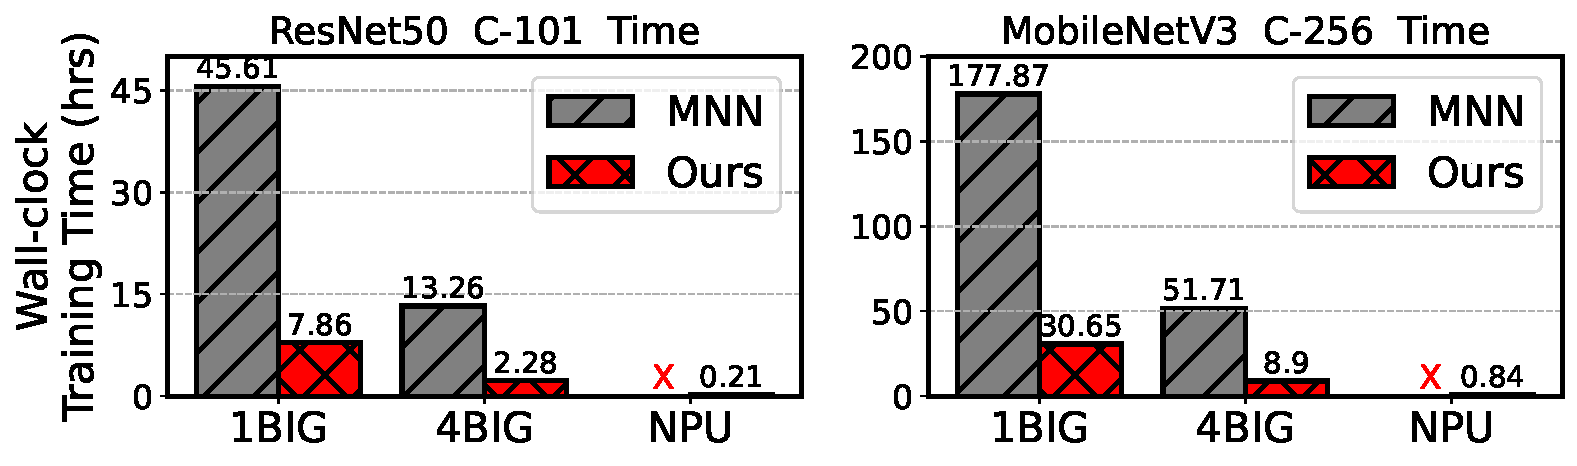
\includegraphics[width=\linewidth]{figs/NPU_time.pdf}
		
		\label{fig:resnet}
	\end{minipage}
	\begin{minipage}[b]{0.96\linewidth}		
            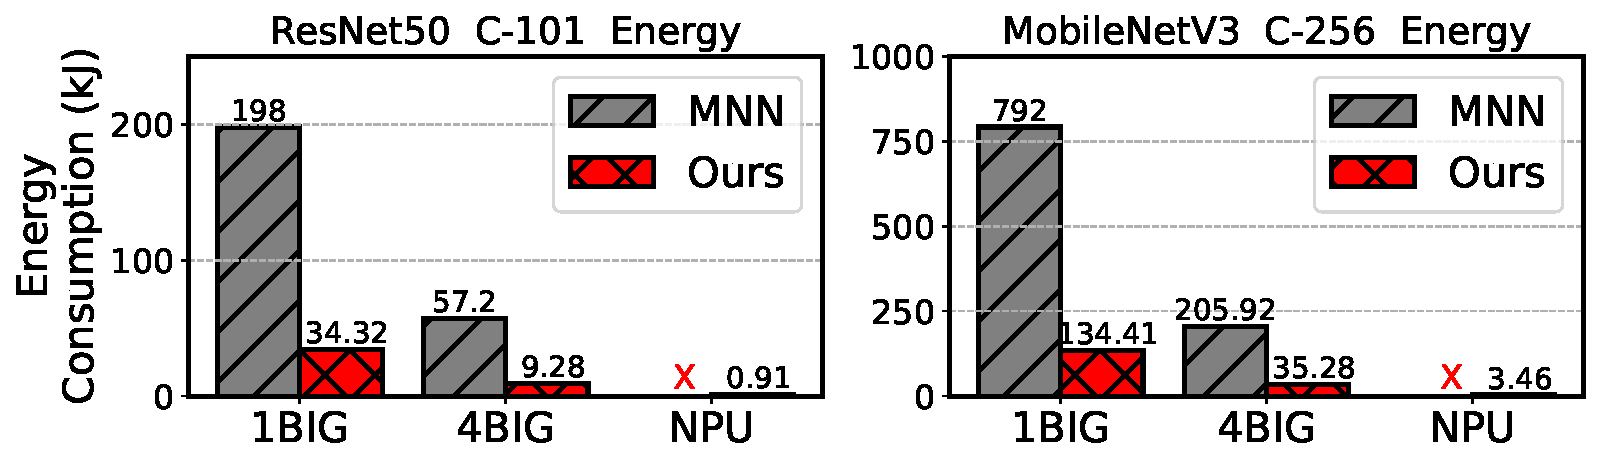
\includegraphics[width=\linewidth]{figs/NPU_energy.pdf}
		
		\label{mbnet}
	\end{minipage}
        
	\caption{Performance on COTS devices with different processors compared to MNN. ``1BIG'', ``4BIG'' and ``NPU'' are run on Huawei Mate30 with 1 CPU big core, 4 CPU big cores and NPU, respectively. ``X'' means not supported.}
         
        \label{fig:NPU}
\end{figure}

Commercial off-the-shelf mobile devices typically integrate various processors into their SoCs for different purposes, such as CPU, GPU, DSP, ISP, NPU, etc.\footnote{Mobile GPUs have been proven unsuitable for DNN training~\cite{das2022enabling}, and DSPs, due to their low-precision (INT8/INT4) computing characteristics, can only be used for training from scratch instead of fine-tuning pre-trained weights~\cite{xu2022mandheling}.} 
While NPUs offer high-precision (FP32/FP16) AI computing ability, their operators and software stacks are closed-source and only inference-friendly (e.g., only high-level non-configurable ABIs available for Kirin NPUs~\cite{Hiai}).
% So there is a gap between NPU and fine-tuning.

Fortunately, \sys's design is NPU-friendly, as its frozen subnets can reuse NPU operators and software stacks for acceleration, while trainable blocks that require weight updates can still be computed on the CPU.
This is a ``syntactic sugar'' at the implementation level, completely orthogonal to the core design of \sys.

We run \sys on a HuaiWei Mate30 smartphone with Kirin 990 half-precision (FP16) NPU, and compare its performance to a popular on-device training framework MNN~\cite{MNN}. 
The default fine-tuning strategy of MNN is full model fine-tuning with 4 CPU big cores.
As is shown in Figure ~\ref{fig:NPU}, with the assistance of key techniques in \sys and NPU offloading, on-device fine-tuning becomes practical and even efficient:
a medium-sized fine-tuning workload (ResNet50, Caltech-101) requires only 0.21 hours and 0.91 kJ of energy, whereas MNN takes 13.26 hours and 57.2 kJ of energy. 
On much larger datasets (Caltech-256), \sys also requires only 0.84 hours and 3.46 kJ of energy.

% Shared setup for the four-condition, full-12-epoch Orin experiment.
% Evidence: ../orin_scheduling/results/feature_20261113_prefetch_full_v2/
\begingroup
\color{blue}
\subsection{Coexisting with Periodic Inference on Jetson Orin}
\label{subsec:orin-periodic}

\begin{table*}[!t]
\color{blue}
\caption{Experiment on Jetson orin with a periodic forground inference workload.}
\label{tab:orin-prefetch}
\centering
\footnotesize
\setlength{\tabcolsep}{4pt}
\renewcommand{\arraystretch}{1.10}
\arrayrulecolor{blue}
\begin{tabular}{@{}lrrrrr@{}}
\toprule
Method & \makecell{Training\\(s)} & \makecell{Training time\\saved (\%)} & \makecell{Accuracy\\(\%)} & \makecell{Inference\\p99 (ms)} & \makecell{Misses\\(\%)} \\
\midrule
FIFO & 737.05 & 0.00 & 91.85 & 26.56 & 0.0042 \\
Reorder & 664.70 & 9.82 & 91.85 & 25.88 & 0.0000 \\
FIFO + prefetch & 569.53 & 22.73 & 91.92 & 26.69 & 0.0134 \\
Reorder + prefetch & 517.06 & 29.85 & 91.39 & 26.02 & 0.0046 \\
\bottomrule
\end{tabular}
\arrayrulecolor{black}
\end{table*}

We test whether reordering training work and computing features ahead of time can speed up background training while foreground inference runs regularly.
We compare four methods: FIFO, Reorder, FIFO with prefetching, and Reorder with prefetching.
FIFO without feature caching is the baseline.
Both optimizations run on the device and leave offline proxy generation and policy training unchanged.

\noindent \textbf{Setup.}
We use a Jetson AGX Orin developer kit with 64\,GB memory in its existing 30\,W power mode.
It runs PyTorch 2.0.0+nv23.05 and CUDA 11.4.
We use the released ResNet50 proxy networks, policy model, and classifier on Caltech-101.
The proxy networks stay frozen, and we train the classifier for 12 epochs with batch size four and an SGD learning rate of 0.001.
All methods use the same models and store tensors in FP32.
We turn off the Python TF32 settings, although the released TorchScript convolution operators still allow TF32 internally.

For the four-method comparison, a foreground inference request arrives every 105\,ms during training.
We measure its response time from its scheduled arrival until the GPU finishes it, including any waiting time.
We set a response-time target of 33.20\,ms before the experiments and process every request.

\noindent \textbf{Scheduling.}
We use the FIFO and Reorder rules in Section~\ref{subsec:reorder}.
All four methods give foreground requests priority and leave a 2\,ms safety margin before the next request.
Reorder looks ahead by up to 128 batches.
Without caching, it stops letting later batches pass the oldest batch after eight such passes.
With caching, only feature computation is reordered; the remaining training work keeps the original batch order.

We estimate how long each operation will take from measured runtimes.
The initial estimate is 1.15 times the 95th-percentile runtime measured without foreground inference.
We then update it to 1.10 times the 95th percentile of the latest 32 measurements, but never below the initial estimate.
For any operation that may update the classifier, we reserve enough time for a full backward update before deciding whether the loss calls for one.

\noindent \textbf{Timing.}
Each reported result comes from one run.
We use a fixed seed to shuffle the run order within each experiment.
Each run starts from the same classifier and routing state and uses the same random seed.
Training time covers all 12 training epochs, including waiting time and scheduling overhead, but excludes evaluation.
Total time also includes the 12 full evaluations and the time needed to finish any remaining foreground requests.
We load the models and prepared images into GPU memory before timing starts.
Initial policy inference, runtime measurements for the starting estimates, and warmup also take place before timing starts.
We check the logs to confirm that all training batches, evaluations, and foreground requests finish, that batches follow the required order, and that the recorded times are consistent.
\par
\endgroup


% Generated only from complete, verified full-12-epoch measurements.
% Evidence: ../orin_scheduling/results/feature_20261113_prefetch_full_v2/
\begingroup
\color{blue}
\noindent\textbf{Prefetching.}
We compute features for upcoming batches before the classifier needs them, as described in Section~\ref{subsec:feature-prefetch}.
We look ahead by up to 128 batches and reserve space for at most 32 batches of features.
A single forward call can process one, two, or four batches that use the same proxy.
The classifier still uses batches of four images and updates in the original order in both prefetch methods.
Each selected training image passes through its assigned proxy once per epoch.
We use each feature once and then release it; the next epoch computes new features.
Evaluation also recomputes its features.
All prefetch work counts toward training time, from preparing the first features to using the last ones.



\noindent\textbf{Results.}
Table~\ref{tab:orin-prefetch} shows the results. Accuracy is measured after epoch 12. A miss means that an inference request takes more than 33.20\,ms to finish.
Compared with FIFO without caching, Reorder alone cuts training time by 9.82\%.
Adding prefetching to FIFO cuts it by 22.73\%, and combining Reorder with prefetching cuts it by 29.85\%.
On top of FIFO with prefetching, reordering feature computation reduces training time by a further 9.21\%.

Final accuracy is 91.85\% for FIFO without caching, 91.92\% for FIFO with prefetching, and 91.39\% for Reorder with prefetching.
The combined method is 0.46 percentage points below the baseline. These runs do not establish that the methods reach the same final accuracy.
The feature buffer uses at most 359.38\,KiB in these runs. This excludes memory for models, inputs, and operator workspaces.


\par
\endgroup


% Generated from verified 12-epoch measurements; do not insert smoke timings.
% Provenance: ../orin_scheduling/period_sweep_protocol.txt
\begingroup
\color{blue}
\noindent\textbf{Varying the foreground inference period.}
We compare FIFO without caching and Reorder with prefetching at request periods of 105, 135, and 180\,ms.
Figure~\ref{fig:orin-period-sweep} reports the time for all 12 training epochs, excluding evaluation, using the same settings as above.
The 105\,ms results are reused from Table~\ref{tab:orin-prefetch}; we run both methods once at each of the other two periods.
Reorder with prefetching reduces training time at all three periods, by 23.97--29.85\% in these runs.
The benefit therefore persists across the tested request periods.


\begin{figure}[!t]
\color{blue}
\centering
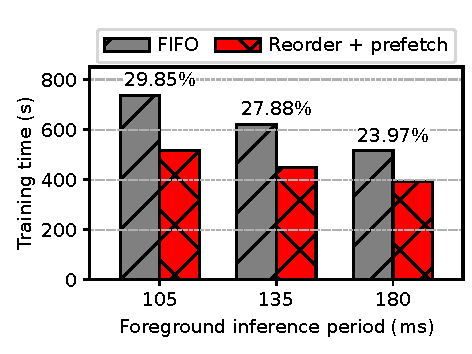
\includegraphics[width=80mm]{figures/orin_period_sweep.pdf}
\caption{Training time under different foreground inference periods. Bars show the time for 12 training epochs, excluding evaluation. Percentages show the reduction relative to FIFO without caching.}
\label{fig:orin-period-sweep}
\end{figure}
\par
\endgroup

